% !TEX encoding = UTF-8 Unicode
%!TEX root = ../Main/thesis.tex
% !TEX spellcheck = en-US
%%=========================================
\documentclass[../Main/thesis.tex]{subfiles}
\begin{document}
\chapter[Hilbert-Huang transform applied to bearing fault detection]{Hilbert-Huang transform for bearing fault detection}
\label{sec:hht}

Most signal decomposition methods such as Fourier transform, impose a-priory basis functions on the signal to be analyzed. In the case of Fourier analysis, the basis functions are trigonometric extensions. Although this implies a rigorous mathematical treatment, the resulting signal decomposition is limited by the mathematical assumptions (\cite{huang98}, \cite{huang08}). Limiting not in the sens of its mathematical truthfulness, rater in it ability to capture all intended salient physical properties of the target signal. Two such assumptions are linearity and stationary. As most phenomena in nature are nonlinear and non stationary, this mathematical approach, although rigorous, lacks an important property: Adaptivity (\cite{huang98}, \cite{huang08}). The latter refers to capturing the intrinsic properties of a signal, without imposing a-priory basis functions, (\cite{huang98}, \cite{huang08}). 
\justify 
The Hilbert-Huang transform (HHT) was precisely developed to deal with nonlinear and non stationary processes, in an adaptive fashion (\cite{huang98}). It combines Hilbert spectral analysis with the so call empirical mode decomposition (EMD), to adaptively decompose a signal into its fundamental components called intrinsic mode functions (IMF), (\cite{huang98}).
The richness of the HHT spans from the analysis of differential equations, to the study of geophysical phenomena, as well as bearings faults detection (\cite{huang08},\cite{li2009}, \cite{yan2006} ,\cite{soualhi2015}, \cite{sallo2019}), and by no mean limited to them.
\justify
 The HHT has been successful applied to the analysis of solutions of nonlinear differential equations, such as the Duffing and the Lorentz equations. The intrinsic frequency, the forcing function and the low intensity subharmonics of the numerical solutions for the nonlinear Duffing equation has been extracted through the EMD process, (\cite{huang98}).
 \justify
  The decomposition of the solutions of Lorentz equation, revealed \say{transient components with different frequencies and damping characteristics}, which agreed with previous studies, (\cite{huang98}). The HHT application to seismic waves propagation, identified high and low frequency seismic waves (\cite{vasudevan2000}). In particular, its decomposition of the seismic waves induced by the 1999 Taiwan earthquake, revealed that \say{the Fourier transform underestimated low frequency energy} (\cite{huang2001}). The Hilbert-Huang transform emerged as a general signal decomposition tool, and in theory can be applied to any signals.
\justify
This chapter presents a new method for bearing fault detection. Its couples the HHT with a robust seasonal trend decomposition method called STL, to detect bearing faults. STL stands for seasonal trend decomposition based on LOESS. In short, the STL decomposes a target signal into a trend and oscillatory components also called  seasonality. The trend is a monotone curve, while the seasonal components are periodic oscillations with a constant period.
\justify
The bulk of this new method, consists of decomposing a target signal into (nearly) mono components signals with the HHT. Furthermore, their respective seasonal components are extracted through the STL. Moreover, the power spectral density of the resulting seasonal component will generate conspicuous frequency peaks, from which bearing failure frequencies can be identified.
\justify
After giving an esquisse of the new method, the remaining of this chapter is organized in the following manner:
 Section \ref{sec:emd} presents the empirical mode decomposition (EMD), which is the back bone of the Hilbert-Huang transform for decomposing a signal adaptively. Section \ref{sec:pulse}, through a concrete case study, demonstrates the efficiency of the new method. It starts by recalling the characteristics of bearing faults such as outer race defect and inner race defect. Furthermore, the experiments that generated the data for this case study are described. Afterwards, the seasonal trend decomposition based on LOESS (STL) is presented, followed by a description of the proposed method for bearing fault detection. Finally, the results of the case study are presented. In closing, section \ref{sec:limitation} presents a summary and discussion of the proposed new method.
\justify



 
 %%%%%%%%%%%%%%%%%%%%%%%%%%%%%%%%%%%%%%%%%%%%%%%%%%%%%%%%%%%%%%%%%%%%%%%%%%%%%%%%%%%%%%%%%%%%%%%%%%%%%%%%
 \section{The Hilbert-Huang transform}
 \label{sec:emd}
 The Hilbert-Huang transform, is the amalgam of the empirical mode decomposition (EMD) and the Hilbert transform.
  The former decomposes a target signal into (nearly) mono component signals, call intrinsic mode functions (IMFs), while the latter enables the extension of a real valued signal to its complex counterpart. Together, the empirical mode decomposition and the Hilbert transform, form the basis for accurately (in the physical and mathematical sens), analyzing amplitude and frequency modulated signal in one hand (\cite{huang98}), and on the other hand, complex signals in general.
\justify
 For a target signal $s(t)$, the goal is to obtained its $n$ fundamental parts (IMFs), denoted here by $s_{j}, j =1,\cdots,n$, through the empirical mode decomposition, such that
\begin{equation}\label{eq:emd-decomposition}
s(t) = \sum_{j=1}^{n}s_{j}(t) + r(t),
\end{equation}
where $r(t)$ is the residual, which is either a constant or a monotone function. The derivation of the intrinsic mode functions $s_{j}$, by means of the empirical mode decomposition, relies on the following key assumptions.
\begin{definition}\label{def:emd}
An intrinsic mode function (IMF) must satisfy the following conditions:
\begin{enumerate}
\item The number of extrema and the number of zero crossing must either equal or differ by one 
\item At any data point, the mean value of the envelope defined using the local maxima and the envelope defined by using the local minima is zero.
\end{enumerate}
\end{definition}
The empirical mode decomposition is an iterative algorithm that generates intrinsic mode functions, each satisfying definition \ref{def:emd}. It can be described as follow:
\begin{enumerate}
	\item Compute the upper and the lower envelope curve of the target signal $s(t)$
	\item In the first iteration ($i=1$), compute the mean $m_{i}(t)$ between the upper and the lower envelope cure of $s(t)$
	\item Compute the first (pseudo) IMF as 
	\begin{equation}\label{eq:proto}
		h_{i1}(t) = s(t)-m_{i}(t).
	\end{equation}
	If $h_{i1}$ satisfies definition \ref{def:emd}, then it is an IMF and it is denoted by 
	\begin{equation}\label{eq:imf}
		c_{i}(t) = h_{i1}(t).
	\end{equation}
	otherwise
	
	\item Set $h_{i1}(t)$ as the input signal and repeat step 1,2 and 3, $k$ time, until $h_{ik}(t)$ satisfies definition \ref{def:emd}.
	\item After finding the first IMF, set the first IMF as input signal and repeat step 1,2,3 and 4 to obtain the remaining IMFs. If an IMF is monotone, set it as the residual and you are done.
\end{enumerate}
 In most function (signal) decomposition methods, a set of predefined $n$ basis functions denote here by $\varphi_{j}(t), j = 1,\cdots,n$, coupled with coefficients $a_{j}$, are used to decomposing a function, say $f(t)$ as 
\begin{equation}\label{eq:basis}
	f(t) = \sum_{j=1}^{n}a_{j}\varphi_{j}(t).
\end{equation}
However, the Hilbert Huang transform will decompose $f(t)$ as 
\begin{equation}\label{eq:hht1}
f(t) = \sum_{j=1}^{n}c_{j}(t) + r(t).
\end{equation}
In equation (\ref{eq:basis}) the basis $\varphi_{j}(t)$ are chosen before hand (a-priory), and the coefficients are computed through an integral or summation operation. A kind of \say{bias} is imposed on the the function $f(t)$. A change of basis function will affect the resulting decomposition. On the hand, in equation (\ref{eq:hht1}) the basis function are directly derived from the properties of the function $f(t)$. This illustrates the concept of adaptivity, central to the Hilbert-Huang transform, which can be seen as basis function agnostic.
\begin{figure}[H] %  figure placement: here, top, bottom, or page
   \centering
   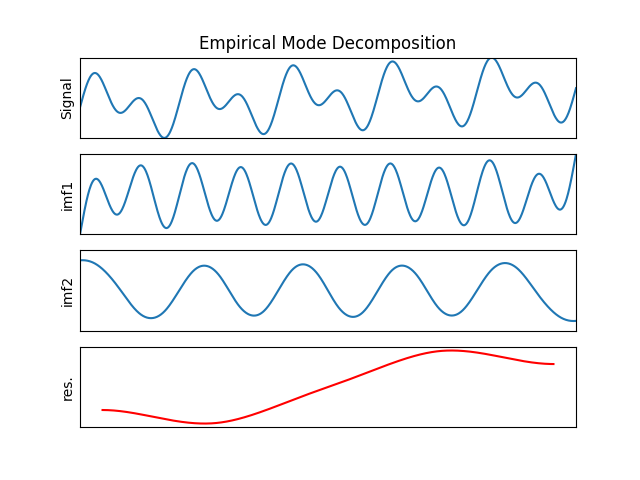
\includegraphics[width=5in]{../fig/imfEMD.png} 
   \caption{The intrinsic mode functions (IMF ) and the residual (in red) generated from the input signal $S(t) = \sin(10 \pi t) + \sin(20 \pi t) $}
   \label{fig:emd3}
\end{figure}
\justify
Figure \ref{fig:emd3} shows the signal  $s(t) = \sin(10 \pi t) + \sin(20 \pi t) $ (top) and its IMFs as well as the residual. The target signal is the superposition of a high and a low amplitude component. Both are recovered by the empirical mode decomposition and labeled as $imf_{1}$ and $imf_{2}$, respectively. The residual component, which contain no oscillations, can be interpreted as noise or uncertainty incurred by the decomposition. 
\justify
The intrinsic mode functions obtained through the EMD process, constitutes an adaptive basis that satisfies the mathematical properties of convergence, completeness, orthogonality and uniqueness, (\cite{huang98}). Furthermore, if $a_{j}(t)$ and $\omega_{j}(t)$ are amplitude and frequency modulation corresponding to IMF $j$, then the original signal $s(t)$ can also be recover as 
\begin{equation}\label{eq:recover2}
s(t) = \Re{\left( \sum_{j=1}^{n}a_{j}(t)\exp\left(i\int\omega_{j}(t)\mathrm{dt}\right)  \right)},
\end{equation} 
where the symbol $\Re(\cdot)$ represents the real part of the expression its encompasses, $i=\sqrt{-1}$, and $n$ is the total number of IMFs obtained from decomposing a signal $s(t)$. Recall that the amplitudes $a_{j}(t)$ and the frequencies $\omega_{j}(t)$ can be computed through the Hilbert transform. An analog representation of equation (\ref{eq:recover2}) in terms of Fourier expansion would be 
\begin{equation}\label{eq:recoverFourier}
s(t) = \Re{\left( \sum_{j=1}^{n}a_{j}\exp\left(i\omega_{j}\right)  \right)},
\end{equation} 
where this time, the amplitude $a_{j}$ and the frequency $\omega_{j}$ are constant. The Hilbert-Huang transform (HHT) offers two different approaches to recover a decomposed signal. The first one is described by equation (\ref{eq:hht1}) and includes the IMFs, while the second approach is given by equation (\ref{eq:recover2}) and includes the instantaneous amplitude and the instantaneous frequency. This gives the HHT a leverage over Fourier transform in nonlinear an non stationary data analysis.
\justify
An important observation can be made, regarding the intrinsic mode functions (IMFs), generated by the empirical mode decomposition (EMD). Figure \ref{fig:input} shows an input vibration signal, which is the superposition of elementary signals. Figure \ref{fig:imfsfreqband} displays the resulting intrinsic mode functions. The first IMF resembles the input function. It contains high frequency components. The sixth IMF, contains lower frequency components than the preceding IMF. And the eleventh IMF contains even lower frequency component then the eighth IMF. Moreover, the empirical mode function behave like a filter bank. Recall that a filter bank decomposes an input target signal into subset signals, each mapping different area in the the spectrum of the original signal. Thus each IMF generated by the EMD corresponds to different frequency range of the input signal.
\begin{figure}[H]
	\centering
	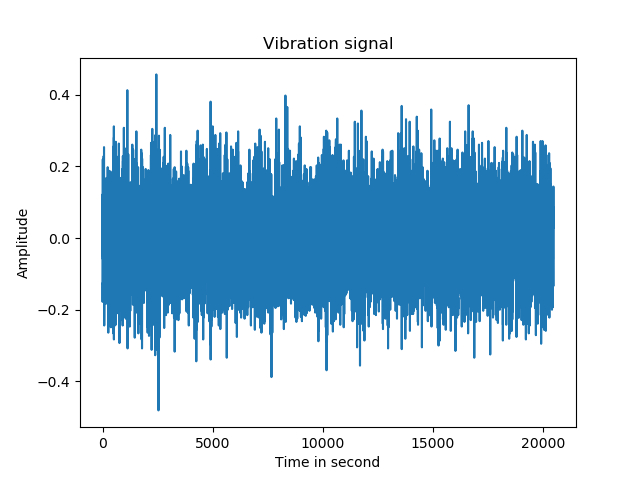
\includegraphics[width=0.7\linewidth]{../fig/input}
	\caption{An input vibration signal}
	\label{fig:input}
\end{figure}
\begin{figure}[H]
	\centering
	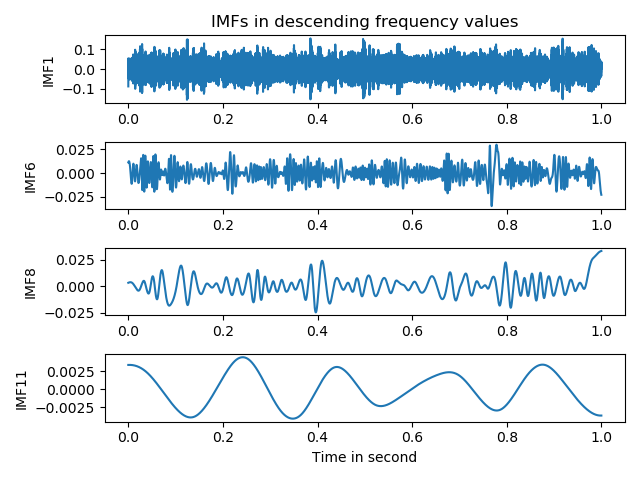
\includegraphics[width=0.7\linewidth]{../fig/imf_freq_band}
	\caption{}
	\label{fig:imfsfreqband}
\end{figure}

%%%%%%%%%%%%%%%%%%%%%%%%%%%%%%%%%%%%%%%%%%%%%%%%%%%%%%%%%%%%%%%%%%%%%%%%%%%%%%%%%%%%%
%%%%%%%%%%%%%%%%%%%%%%%%%%%%%%%%%%%%%%%%%%%%%%%%%%%%%%%%%%%%%%%%%%%%%%%%%%%%%%%%%%%%%
%%%%%%%%%%%%%%%%%%%%%%%%%%%%%%%%%%%%%%%%%%%%%%%%%%%%%%%%%%%%%%%%%%%%%%%%%%%%%%%%%%%%%

\section{Application to bearing fault detection: a case study}
\label{sec:pulse}
In this section, the proposed new method is applied to a case study, in order to demonstrate its ability in detecting bearing failure. As a reminder, Figure \ref{fig:bearing-architecture} shows a geometry of a bearing, with different parts.
\begin{figure}[H] %  figure placement: here, top, bottom, or page
   \centering
   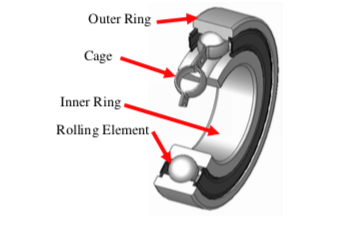
\includegraphics[width=4in]{../fig/bearing.png} 
   \caption{Geometrical representation of a bearing}
   \label{fig:bearing-architecture}
\end{figure}
\justify
A fault occurring at the outer ring is called a ball pass frequency outer ring (BPFO) defect. While a fault in the inner ring occurs at a frequency called ball pass inner race frequency (BPFI). They are given in Hz in terms of the bearing geometrical characteristics an the rotating speed of the shaft as
\begin{equation}\label{eq:bpfo2}
BPFO = \frac{nb}{2}R\left(1-\frac{BD}{PD}\cos\left(\beta\right)  \right) \nonumber
\end{equation}
\begin{equation}\label{eq:bpfi2}
BPFI = \frac{nb}{2}R\left( 1 +  \frac{BD}{PD}\cos\left(\beta\right)   \right),
\end{equation}
where R is the rotating speed of the motor on which the bearing is attached. nb is the number of rolling elements (balls), BD is a rolling element diameter. The pitch diameter PD is half the height of the inner ring, and the contact angle $\beta$ is the angle formed when a rolling element touches the cage. 
\justify
The data and the experimental setup used for this case study were described in chapter 2. In this setup, four bearings are mounted on a motor rotating at 2000 rotations per minutes (33.3 Hz). In the first experiment the motor runs until
bearing number 3 is severely damaged with inner race defect, while in the second experiment outer race defect occurs in bearing number 1. For each experiment, successive vibration signals where obtained, with a sample rate of 20 $KHz$ and corresponding Nyquist frequency of 10 $KHz$ (half the sampling rate). The Nyquist frequency define a lower bound limit in order to avoid aliasing, which is a loss of information due to under sampling. That is, if the sample contain frequency components that are higher then the Nyquist frequency, those frequency components wont be able to be seen.

\justify
\subsection{Seasonal Trend decomposition based on Loess (STL)}
The STL sequentially applies the locally estimated scatter plot smoother (LOESS) in order to obtain cyclical and trend components of a signal (\cite{Cleveland-1979}, \cite{Cleveland-et-al-1988}). Here a cyclical component is a periodically occurring pattern in a signal. The  locally estimated scatter is a non parametric curve fitting procedure.  It can be used for \say{Data exploration, diagnostic checking of parametric models and provides a non parametric regression surface}.
If $s(t)$ is a signal, the goal is to obtained the decomposition 
\begin{equation}
s(t) = T_{r}(t) + C_{y}(t) + R_{res}(t),
\end{equation} 
where $T_{r}(t)$ an $C_{y}(t)$ are the trend and cyclical components, and $R_{res}(t)$ is the residual obtained from subtracting  the trend and the cyclical component from the signal. The key ingredient in the STL, is the locally estimated scatterplot smoother procedure. The latter being a non parametric regression method, does not rely on any a-priory assumption on the shape of the curve that needs to be fitted. It therefore provides a flexible approach to curve fitting, by capturing local, as well as global characteristics of a signal. A detailed account of the STL can be found in  (\cite{Cleveland-et-al-1990}).
\justify
One  professed limitation of the empirical mode decomposition, is refer to as mode mixing. The resulting intrinsic mode functions (IMFs) are not exactly mono components. Being mono component means that each IMF should be a sinusoidal with one frequency characteristics. Having for example an IMF with high frequency and low frequency components will be refer to as mode mixing. In this thesis, the STL is used to address the mode mixing issue. This approach advantages is two folded: In one hand it solves the mode mixing issue by extracting the dominant frequency characteristic, and on the other hand its generates a clear frequency spectrum, as will be shown later.
%%%%%%%%%%%%%%%%%%%%%%%%%%%%%%%%%%%%%%%%%%%%%%%%%%%%%%%%%%%%%%%%%%%%%%%%%%%%%%%%%%%%%%%%%%%%%%
%%%%%%%%%%%%%%%%%%%%%%%%%%%%%%%%%%%%%%%%%%%%%%%%%%%%%%%%%%%%%%%%%%%%%%%%%%%%%%%%%%%%%%%%%%%%%%

\subsection{Results }
In this section we apply the empirical mode decomposition followed by the seasonal trend decomposition based on LOESS to extract pulses emitted by a failed bearing.
Figure \ref{fig:pulse} shows a flow diagram, describing the methodology to obtaining pulse signals emitted from a bearing with ball pass frequency outer race defect. An input signal goes through the empirical mode decomposition to generate intrinsic mode functions. Furthermore, the STL is applied on the intrinsic mode functions to generate a periodic signal which looks like a pulse. And finally, the power spectral density of the resulting signal is approximated by the periodogram method.
\justify
The power spectral density is technically the power or energy distribution of the autocovariance function (ACF) frequency spectrum. (\cite{stoica2004}). The autocovariance function of a signal $s(t)$ is defined by 
\begin{equation}
	ACF(s(t)) = E\left[ s^{*}(t)s(t-k) \right] = COV\left(s(t), s^{*}(t-k)\right)\quad k = 0,1, \cdots
\end{equation}
where $E(\cdot)$ is the expectation or mean, COV($\cdot$) is the covariance and $s^{*}(t)$ is the complex conjugate of $s(t)$. The covariance of the signal $s(t)$ and its complex conjugate measures their joint variability. Thus the autocovariance function is a sequence of covariance between the signal and its complex conjugate. Now, the power spectrum density (PSD) of a signal s(t) can be defined by (\cite{stoica2004})
\begin{equation}\label{eq:psd}
	PSD\left(s(t)\right) = E\left[ \frac{1}{N} \left\vert \sum_{t=1}^{N} s(t)e^{-iwt}\right\vert^{2}   \right]
\end{equation}
where $N$ is a large integer, $i=\sqrt{-1}$, $E(\cdot)$ is the expected value, and $\omega$ is the angular frequency. The estimation $\widehat{PSD}$
\begin{equation}
		\widehat{PSD}\left(s(t)\right) =  \frac{1}{N} \left\vert \sum_{t=1}^{N} s(t)e^{-iwt}\right\vert^{2}
\end{equation}
of the power spectral density in equation (\ref{eq:psd}) is called the periodogram.
\begin{figure}[H]
\begin{tikzpicture}
  [node distance=.8cm,
  start chain=going below,]
     \node[punktchain, join] (intro) {\textcolor{blue}{Input signal}};
     \node[punktchain, join] (probf)      {\textcolor{violet}{EMD}};
     \node[punktchain, join] (investeringer)      {\textcolor{blue}{IMFs}};
     \node[punktchain, join] (perfekt) {\textcolor{violet}{STL}};
     \node[punktchain, join] (perfekt) {\textcolor{blue}{Pulse signal}};
     %\node[punktchain, join, ] (emperi) {Fast Fourier transform};
     % \node (asym) [punktchain ]  {Asymmetrisk information};
      \begin{scope}[start branch=venstre,
        %We need to redefine the join-style to have the -> turn out right
        every join/.style={->, thick, shorten <=1pt}, ]
        \node[punktchain, on chain=going left, join=by {->}] (risiko) {\textcolor{blue}{Power spactrum density}};
      \end{scope}
      \begin{scope}[start branch=hoejre,]
      %\node (finans) [punktchain, on chain=going right] {Det finansielle system};
    \end{scope}
    \end{tikzpicture}
  \caption{Schematic description of the methodology to obtaining a pulse like signal containing all diagnostic information for bearing fault detection}
   \label{fig:pulse}
\end{figure}
\justify
Figure \ref{fig:imf} shows the first, seventh and twelfth IMF of an input vibration signal for a bearing. The first few IMFs correspond to high frequency components in the original signal, and lower frequency components are represented by higher IMF. Here the first IMF ($IMF_{1}$) represents the components with the highest frequency. As discussed earlier, mode mixing can be seen in $IMF_{7}$, where high and low frequency components are intertwined. The $IMF_{12}$ on the other hand represent low frequencies components of the target vibration signal.
Figure \ref{fig:emd-stl} shows  the input vibration signal (top), its fifth IMF (middle) and its seasonal component (bottom) obtained by applying the seasonal trend decomposition by LOESS (STL).   
\justify
The seasonal part of the fifth IMF is periodic and has a pulse like configuration. This is consistent with a bearing having a fault located in the inner ring. As the bearing rotates, when the bearing roller elements (balls) strike the faulty area, the amplitude increase rapidly, before decaying. This process is repeated throughout the bearing operation state, and is well captured by the proposed method. The pulses obtained represent the signal emitted by the faulty bearing.

\begin{figure}[H] %  figure placement: here, top, bottom, or page
	\centering
	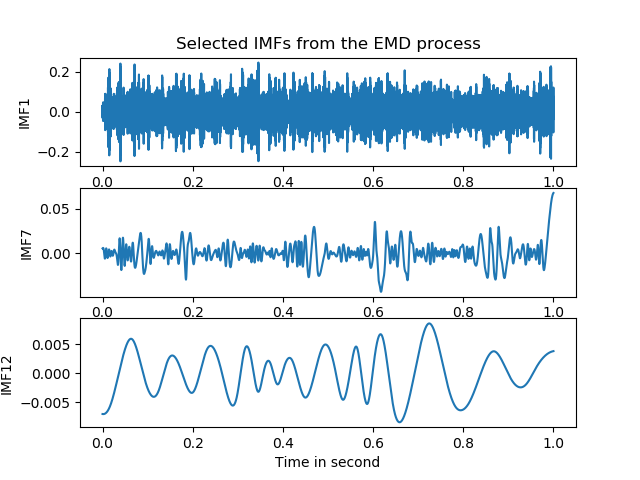
\includegraphics[width=6in]{../fig/selected_imf.png} 
	\caption{Intrinsic mode function number 1, 7 and 12, generated by the empirical mode decomposition}
	\label{fig:imf}
\end{figure}
\justify

\begin{figure}[H] %  figure placement: here, top, bottom, or page
   \centering
   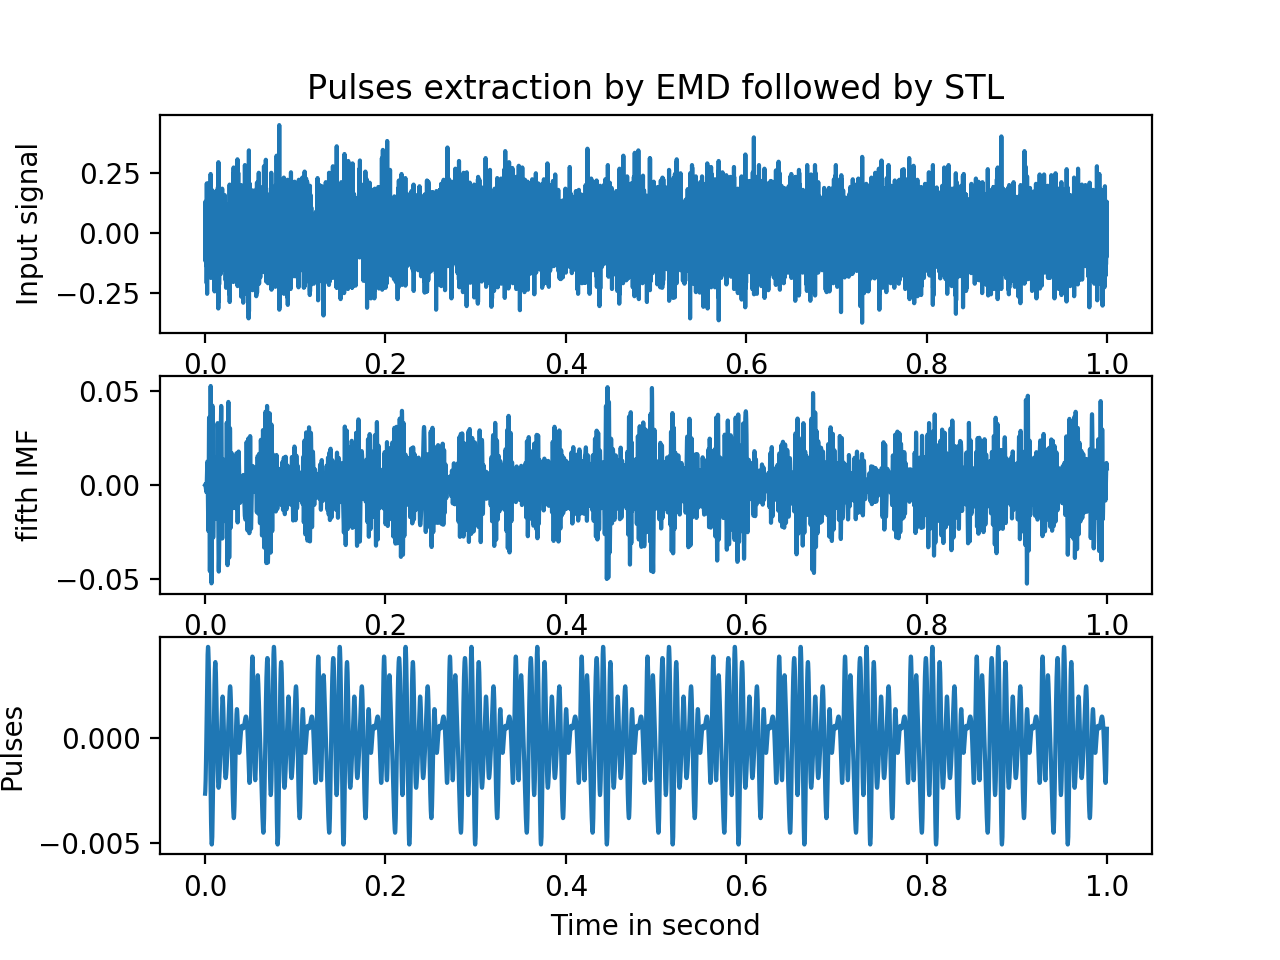
\includegraphics[width=6in]{../fig/emd-stl.png} 
   \caption{ A pulse signal extracted by applying EMD followed by STL. The top graph represents the vibration time signal. The middle graph is the fifth intrinsic mode function. The bottom graph is the signal resulting from applying the STL on the IMF. The pulses represents the periodic high frequency signal emitted by bearings defects.}
   \label{fig:emd-stl}
\end{figure}
\justify
The following sections bellow, show the periodogram, which is the estimation of the power spectral density, of the first intrinsic mode function of faulty bearing. The aim is to identify faulty frequency in the outer and inner ring of a defect bearing.

\subsubsection{Ball pass frequency outer race detection} 
 \begin{figure}[H]
 	\centering
 	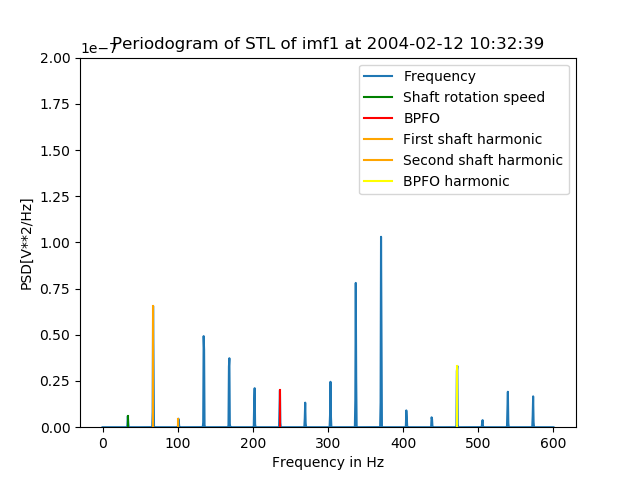
\includegraphics[width=0.8\linewidth]{../fig/periodogram_bpfo/start_imf1_bpfo}
 	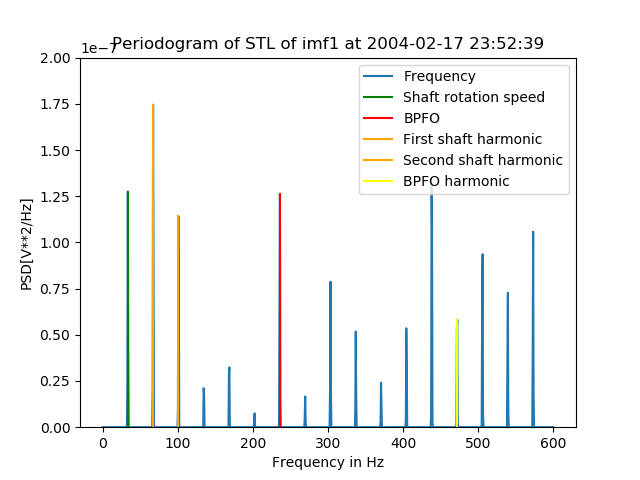
\includegraphics[width=0.8\linewidth]{../fig/periodogram_bpfo/end_imf1_bpfo}
 	\caption{Periodogram of the pulse signal obtained from the first IMF, at the beginning (top) and the end (bottom) of experiment number 2}
 	\label{fig:startimf1bpfo}
 \end{figure}
\justify
Figure \ref{fig:startimf1bpfo} shows the periodogram of the seasonal component from the first IMF obtained at the beginning (top) and at the end of experiment number 2. The periodogram shows conspicuous frequency peaks. At the beginning, the ball pass outer race frequency defect (236.4 Hz) is visible with a relatively low amplitude. At the end, there is a relatively high increase in the outer race frequency defect, showing an increase in the severity of the damage incurred by the bearing.
\justify
In addition, the rotating speed (33.3Hz) of the machine shaft is visible in both cases. Harmonics of the defect frequency ar also visible. And the magnitude of the harmonics have also increased, as the bearing defect is accentuated. Recall that harmonics are characteristics of bearing outer race defect, and they are integer multiple of the defect frequency (236.4 Hz) and machine speed (33.3).

\justify
The difference between the theoretical value of the ball pass outer frequency defect (236.4 Hz) and the one from the periodogram (236.03 Hz) is about 0.16$\%$. While the difference between the theoretical shaft frequency (33.33 Hz) and the on the periodogram (33.63 Hz) is about 0.9 $\%$. This shows that the proposed method is quit accurate in detecting important diagnostic information from the vibration signal.
\justify
In general, the pulse signals extracted from the intrinsic mode functions through the STL method, had more diagnosis information for the fist two IMFs. This can been seen in Figure \ref{fig:startimf2bpfo}, which shows the periodogram of the pulse signals extracted from the second intrinsic mode function, at the beginning and at the end of experiment 2. At the end of the experiment, the energy of the ball pass outer race defect and its harmonic increased.
\justify
%The highest intrinsic mode functions contain mostly the shaft rotation speed and sometimes its harmonics. This can been seen in Figure \ref{fig:startimf8shaft} which shows the Peridogram of the pulse signals obtained from IMF number 8, at the beginning (top) and at the end (bottom) of experiment number 2.

 \begin{figure}[H]
	\centering
	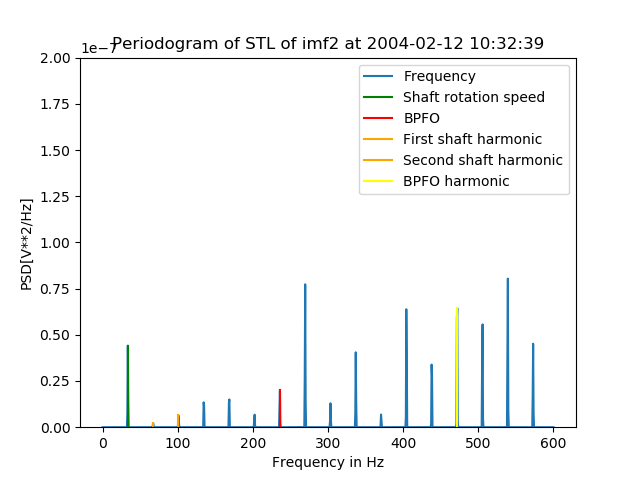
\includegraphics[width=0.8\linewidth]{../fig/periodogram_bpfo/start_imf2_bpfo}
	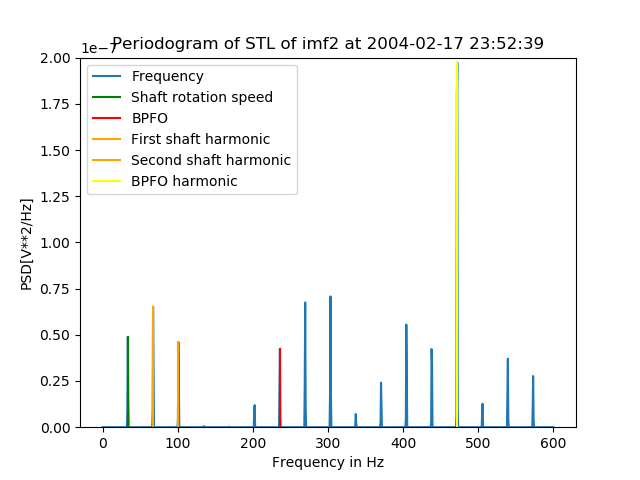
\includegraphics[width=0.8\linewidth]{../fig/periodogram_bpfo/end_imf2_bpfo}
	\caption{Periodogram of the pulse signal obtained from the second IMF, at the beginning (top) and the end (bottom) of experiment number 2.}
	\label{fig:startimf2bpfo}
\end{figure}

 \begin{figure}[H]
	\centering
	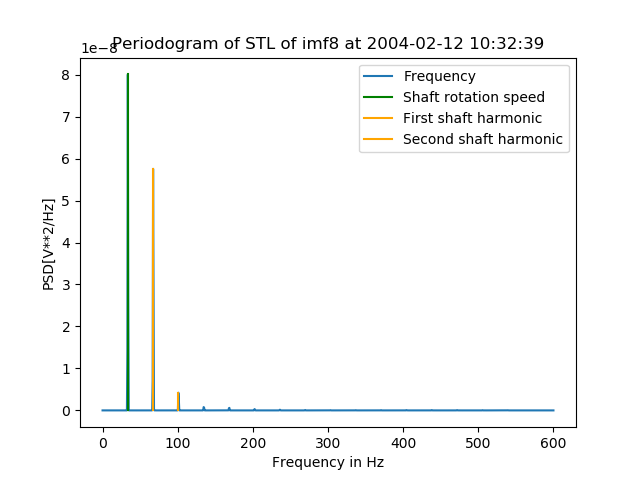
\includegraphics[width=0.8\linewidth]{../fig/periodogram_bpfo/start_imf8_shaft}
	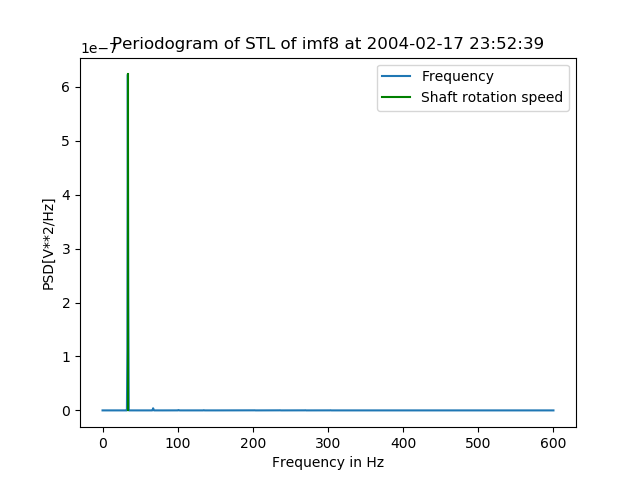
\includegraphics[width=0.8\linewidth]{../fig/periodogram_bpfo/end_imf8_shaft}
	\caption{Periodogram of the pulse signal obtained from IMF number 8, at the beginning (top) and the end (bottom) of experiment number 2.}
	\label{fig:startimf8shaft}
\end{figure}
\justify
\subsubsection{ Ball pass inner race frequency detection }

\begin{figure}[H]
	\centering
	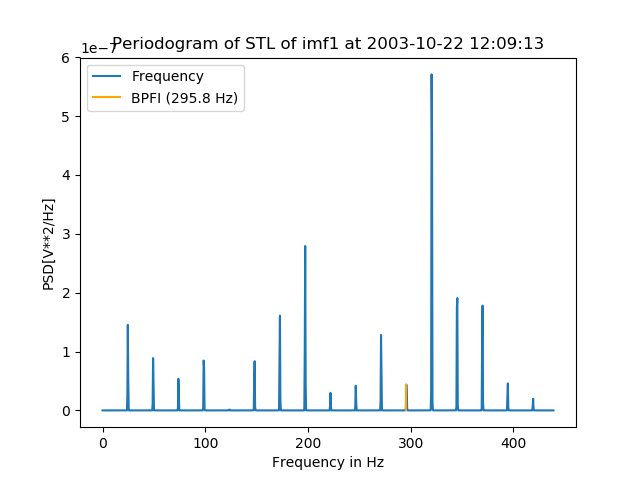
\includegraphics[width=0.8\linewidth]{../fig/periodogram_bpfi/start_imf1_bpfi}
	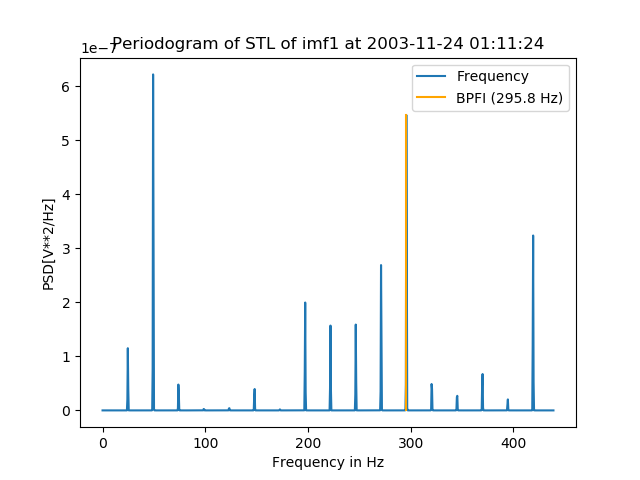
\includegraphics[width=0.8\linewidth]{../fig/periodogram_bpfi/end_imf1_bpfi}
	\caption{Periodogram of the pulse signal obtained from IMF number 1, at the beginning (top) and the end (bottom) of experiment number 1.}
	\label{fig:startimf1bpfi}
\end{figure}
\justify
Figure \ref{fig:startimf1bpfi} shows the periodograms obtained from the pulse signals of the first intrinsic mode functions at the start (top) and at the end (bottom) of experiment number 1. The inner race defect frequency is visible in both cases.
However, the shaft frequency is not visible. The difference between the theoretical value of the BPFI (296.8 Hz) and the detected value (295.8) is about 0.33 $\%$.
\section{Summary}
\label{sec:limitation}
The proposed method consists of transforming a vibration signal to a pulse like signal, which contains all diagnostics information in terms of bearing failure detection. In particular, the outer race and the inner race defect. The present method uses the empirical mode decomposition (EMD), followed by the seasonal trend decomposition method based on Loess (STL). The former is a signal decomposition method suited for non stationary and non linear signal, while the letter extracts periodic components from a signal.
\justify
Together they are able to generate a noise less periodogram which contains relevant frequency information for bearing fault detection. The periodogram approximates the power spectral density (PSD) of a signal. The PSD is the energy distribution of frequencies components of a signal.
By applying the proposed method, it was possible to identify conspicuous outer and inner race defect frequencies, as well as the roation frequency of the machine shaft, in a periodogram pertaining to a bearing undergoing failure.








\blankpage
\end{document}

